\documentclass[presentation,english]{beamer}
\usepackage[utf8]{inputenc}
\usepackage{babel}
\usepackage{fixltx2e}
\usepackage{graphicx}
\usepackage{longtable}
\usepackage{float}
\usepackage{wrapfig}
\usepackage{soul}
\usepackage{textcomp}
\usepackage{marvosym}
\usepackage{wasysym}
\usepackage{latexsym}
\usepackage{amssymb}
\usepackage{hyperref}
\tolerance=1000
\usepackage{listings}
\usepackage[iso]{isodate}
\usepackage{pgfgantt}
\usepackage{caption}

\title[Peer-to-Peer Incentives]{Incentives for Cooperation in a Peer-to-Peer
Name-Lookup Service}
\author{Marc Lehmann}
\subtitle{Initial Master Talk}
\date{\today}


\usetheme{Comsys}
% Adjust the title font size, because my title spans 3 lines otherwise.
\setbeamerfont{title}{size*={16}{26.4},series=\bfseries}

\begin{document}

\setbeamertemplate{footline}[empty]
\begin{frame}
  \titlepage
\end{frame}

\setbeamertemplate{footline}[comsys]

\begin{frame}{Overview}
  \begin{itemize}
    \item Mapping names (IDs) to IPs
    \item Like DNS, but more general (flat namespace)
    \item Decentralized service (DHT)
    \item Goal: get everyone who uses it to contribute
  \end{itemize}
\end{frame}

\begin{frame}{Motivation}
  \begin{itemize}
    \item DNS basically centralized: typical user's DNS lookups go through one
          server
    \item Privacy concerns
    \begin{itemize}
      \item DNS server gets a lot of information about what servers a user
            contacts
      \item Can build user profiles
      \item Can become target for others who want to build profiles
    \end{itemize}
    \item Could be dealt with via (computationally) private information
          retrieval ((c)PIR)
    \item But is impractical: server has to process entire database for every
          request
  \end{itemize}
\end{frame}

\begin{frame}{Motivation}
  \begin{itemize}
    \item Instead of trusting a central server, spread requests to many
          different nodes
    \item Each of them only gets a small amount of data, harder to build a
          profile
    \item Requires users of the service also offering service
    \item Assume people are selfish and rational: incentivize them with better
          service
  \end{itemize}
\end{frame}

\begin{frame}{Distributed Hash Table}
  \begin{itemize}
    \item Store ID-IP mappings in a structured DHT (Kademlia, P-Grid)
    \item Peers pick a prefix and are responsible for items with that prefix
    \item Peers are in contact with others responsible for the same items
    \item For other prefixes: know other peers closer to them
  \end{itemize}
  \begin{figure}
    \centering
    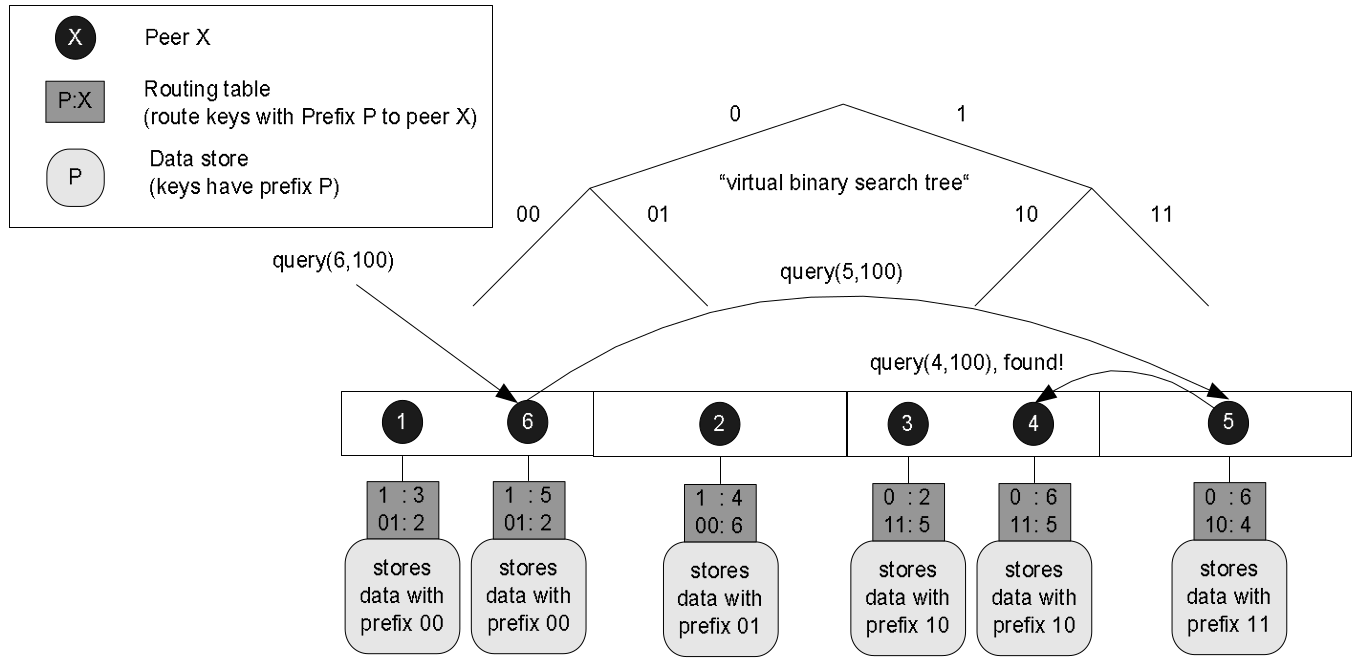
\includegraphics[width=0.5\textwidth]{p-grid}
    \caption*{\tiny From \emph{P-Grid: A Self-organizing Structured P2P System}}
  \end{figure}
\end{frame}

\begin{frame}{Incentives}
  \begin{itemize}
    \item Only leverage: users want good service
    \item Users who don't contribute need to be given lower level of service
          (responses deliberately delayed)
    \item Peers need to know what level of service to grant: reputation system
    \item Track how well peers contribute (abide by the rules)
    \item E.g. point system (credit-debit/credit-only)
  \end{itemize}
\end{frame}

\begin{frame}{Related Work}
  \begin{itemize}
    \item Free-riding given cheap pseudonyms
    \item Cooperation incentives have been investigated
    \item Reputation tracking seen as given, or deferred to a DHT
    \item Alternative reputation systems: tokens
    \item Collusion detection based on typical behavior
  \end{itemize}
\end{frame}

\begin{frame}{Reputation Tracking}
  \begin{itemize}
    \item Requests can come from anyone (that's the point)
    \item Need to be able to find out anyone's reputation
    \item Storing locally impractical for large networks
    \item Storing in a DHT is too slow
  \end{itemize}
\end{frame}

\begin{frame}{Reputation Tracking}
  \begin{itemize}
    \item Peers form small groups in which they forward queries ("the second
          kind")
    \item Reputation tracked in those groups (locally)
    \item Short-lived for privacy, but long enough that trust can grow
  \end{itemize}

  \begin{figure}
    \centering
    \begin{tikzpicture}
      \begin{scope}[every node/.style={draw}]
        \node[color=red] (A) at (0:2) {P: 001};
        \node[color=blue] (B) at (45:2) {P: 001};
        \node[color=red] (C) at (90:2) {P: 001};
        \node[color=blue] (D) at (135:2) {P: 010};
        \node[color=green] (E) at (180:2) {P: 010};
        \node[color=blue] (F) at (225:2) {P: 101};
        \node[color=red] (G) at (270:2) {P: 101};
        \node[color=green] (H) at (315:2) {P: 101};
      \end{scope}

      \path (A) edge[thick,dashed,bend right=15] (B);
      \path (B) edge[thick,dashed,bend right=15] (C);
      \path (A) edge[thick,dashed,bend left=15] (C);
      \path (D) edge[thick,dashed,bend right=15] (E);
      \path (F) edge[thick,dashed,bend right=15] (G);
      \path (G) edge[thick,dashed,bend right=15] (H);
      \path (F) edge[thick,dashed,bend left=15] (H);
      \path (A) edge[thick,color=red,bend left=20] (C);
      \path (C) edge[thick,color=red] (G);
      \path (A) edge[thick,color=red,bend right=15] (G);
      \path (B) edge[thick,color=blue] (D);
      \path (D) edge[thick,color=blue,bend left=15] (F);
      \path (B) edge[thick,color=blue] (F);
      \path (E) edge[thick,color=green] (H);
    \end{tikzpicture}
  \end{figure}
\end{frame}

\begin{frame}{Goal of the Thesis}
  \begin{itemize}
    \item Is such an incentive system possible, assuming selfish peers?
    \item Is there inflation or deflation of reputation?
    \item Could the resulting system be practically useful?
    \item What's the overhead?
  \end{itemize}
\end{frame}

\begin{frame}{Methodology}
  \begin{itemize}
    \item Simulate with SimPy/OMNeT++
    \item Focus on behavior of peers, not the network
    \item Let them update their strategy
    \item Observe how peers' strategies change and what level of service is
          achieved
  \end{itemize}
\end{frame}

\begin{frame}{Methodology}
  \begin{itemize}
    \item Optional: analytical, game-theoretic solution
    \item Are there equilibria?
    \item Are they always reached?
    \item What is their social value?
  \end{itemize}
\end{frame}

\begin{frame}{Timeline}
  \begin{ganttchart}[
    vgrid={*9{draw=none}, dotted},
    x unit=0.035cm,
    title label font=\tiny\bfseries,
    bar label font=\tiny\bfseries
  ]{1}{250}
  \gantttitlelist{1,...,25}{10} \\
  \ganttbar{Implementation}{1}{40}
  \ganttbar{}{51}{80}
  \ganttbar{}{96}{125} \\
  \ganttbar{Evaluation}{41}{60}
  \ganttbar{}{76}{105}
  \ganttbar{}{116}{140}
  \ganttbar{}{161}{190} \\
  \ganttbar{Writing}{161}{230} \\
  \ganttbar{Buffer}{231}{250}
  \end{ganttchart}
\end{frame}

\begin{frame}
\end{frame}

\begin{frame}{Why do we need incentives?}
  \begin{itemize}
    \item Maybe we don't
    \item "Just distribute software that contributes to the DHT, people will be
          too lazy to change it for a small benefit"
          \begin{itemize}
            \item Some alternative implementation may opt to leave it out
            \item Maybe for performance, maybe for security
          \end{itemize}
    \item Assume the worst case, be ready for reality
    \item Just nice to know if it would work
  \end{itemize}
\end{frame}

\begin{frame}{Some more questions}
  \begin{itemize}
    \item Could an attacker still collect information by joining many groups (of
          the second kind)?
    \item How many defectors can the system tolerate?
    \item How many malicious peers can the system tolerate?
    \item How many peers behaving too generously can the system tolerate?
    \item How annoying is starting out with no reputation anywhere?
    \item What about peers that are rarely online?
  \end{itemize}
\end{frame}

\begin{frame}{Some more questions}
  \begin{itemize}
    \item What's a sensible number of groups for a peer to be in?
    \item What's a good group size?
    \item How are groups connected?
    \item Can the rules of the reputation system be changed at run time?
    \item If some ID-IP mappings are more popular than other, won't less popular
          ones be neglected because they offer a smaller benefit?
  \end{itemize}
\end{frame}

\end{document}
